\documentclass{article}
\usepackage[table]{xcolor}
\usepackage{float}
\usepackage{array}
\usepackage{graphicx}
\usepackage[spanish, es-tabla]{babel}
\usepackage[utf8]{inputenc}
\usepackage{csquotes}
\usepackage[margin=1.55cm]{geometry}
\usepackage[backend=biber]{biblatex}
\setlength{\parskip}{1em}
\parindent 0px
\addbibresource{references.bib}

\newcolumntype{P}[1]{>{\centering\arraybackslash}p{#1}}
\newcolumntype{M}[1]{>{\centering\arraybackslash}m{#1}}

\newcommand\cronograma{
	\cellcolor[HTML]{0bd47d}
}

\newcommand\signature{
\noindent\begin{minipage}{10cm}
    \noindent\vspace{3pt}\par
    Firma: \rule{7cm}{1pt}
    \noindent\vspace{15pt}\par
\end{minipage}}

\begin{document}

\begin{center}
	\begin{Large}
		\textbf{Aplicación móvil gamificada de aritmética}
	\end{Large}

	\textbf{Trabajo Terminal No.}

	Alumnos: Pineda Vieyra Itzcoatl Rodrigo, Mothelet Delgado Izaird Alexander

	Directores: Ruiz Ledesma Elena Fabiola, Lorena Chavarría Baez

	e-mail: itzcoatlpv@gmail.com
\end{center}

\section*{Resumen}
La intervención educativa requiere de una previa comprensión de la adquisición
y desarrollo de la competencia aritmética que está en la base de todas las 
posteriores dificultades y trastornos del aprendizaje matemático. Hay dificultades 
que pueden surgir a lo largo de este proceso, lo que repercute en la resolución de 
ejercicios y problemas matemáticos avanzados. Por lo que el desarrollo de la destreza 
operatoria aritmética es fundamental para que el estudiante pueda enfrentar con éxito  
situaciones más complejas en el campo de la Matemática, además, se requiere motivar al 
estudiante al desarrollar trabajo operatorio aritmético, ya que en ocasiones su desarrollo 
puede resultar monótono y aburrido. Para ayudar al desarrollo de la destreza operatoria 
de los estudiantes se propone una aplicación gamificada móvil que promueva la resolución 
de ejercicios Aritméticos.

\textbf{Palabras clave} - Aritmética, Gamificación, Motivación, App móvil.

\section{Introducción}
La Aritmética como la Geometría son de las disciplinas matemáticas más antiguas y 
necesarias en la historia del género humano\cite{coronado2014estudio}. Su utilización 
funcional es requerida para las personas que participamos de esta sociedad, como 
medio de comunicación y comprensión de multitud de fenómenos que nos rodean, es por 
ello que el desarrollo de la destreza operatoria aritmética es una de las habilidades 
más necesitadas en la alfabetización socio instrumental. Los niveles de fracaso en el 
aprendizaje matemático son preocupantes, especialmente en los últimos cursos de 
escolaridad obligatoria (secundaria).  Los resultados de estudios internacionales 
como el Programa Internacional para la Evaluación de Alumnos de la OCDE 
(PISA)\cite{oecd2014what,oecd2016low}, muestran que el aprendizaje matemático es el 
que presenta mayor porcentaje de fracaso\cite{coronado2016academic, mullis2016timss}. 
El cálculo es un componente esencial en la resolución de problemas aritméticos, 
y éste es uno de los contenidos más importantes de las matemáticas, junto a la geometría, 
la medida o la probabilidad. Es por ello que un elevado porcentaje de las dificultades de 
aprendizaje de las matemáticas tiene un origen aritmético, donde el cálculo representa un 
papel esencial\cite{orrantia2006dificultades}.  Las habilidades numéricas y aritméticas 
son predictores críticos del futuro éxito o fracaso académico 
matemático\cite{rodriguez2017marcadores}.  


La aritmética es la parte de la matemática, referida a los números y a las operaciones 
y cálculos básicos que pueden realizarse con ellos: adición, sustracción, multiplicación 
y división. Su desarrollo es fruto de la madurez cognitiva del sujeto en la interacción 
con los objetos y la mediación de los instrumentos socioculturales de su contexto.  
El conocimiento de las operaciones básicas surge a partir de los aprendizajes informales 
y formales del conocimiento matemático. Las investigaciones cognitivas que han estudiado el 
desarrollo de las habilidades para el cálculo, han establecido que esta competencia requiere 
de la integración de una serie de esquemas protocuantitativos\cite{resnick1989developing,resnick1987learning}
con la experiencia de contar\cite{fuson1992research}.  Esas estrategias de conteo que 
se utilizan inicialmente para sumar y restar, se van haciendo más complejas con el uso 
y la práctica, ampliándose a las operaciones de multiplicar y dividir, cuya práctica las 
hace interiorizarse en esquemas de memoria que posibilitarán posteriormente la recuperación 
de hechos numéricos (desde la memoria a  largo plazo semántica) para la solución de operaciones 
de cálculo\cite{fuson1992research,godino2009sentido,fuson1988children}.


La problemática que se pretende atacar es la necesidad de fortalecer la destreza 
operatoria aritmética de los estudiantes de nivel medio y superior\cite{gusty2005importance,tariq2002decline}, 
lo cual es importante para el desarrollo del pensamiento matemático de los estudiantes.


Con este proyecto se pretende ayudar al desarrollo de la destreza operatoria en la 
resolución de ejercicios aritméticos con números enteros y fraccionarios, haciendo 
uso de ciertos componentes de la gamificación (Logros) y mecánicas (Competición). 
Como futuros ingenieros en sistemas computacionales tenemos la responsabilidad de usar 
las habilidades para un beneficio social, por lo que deseamos unir esfuerzos para apoyar 
al estudiante a mejorar su destreza operatoria.


La gamificación no consiste en enseñar por medio de juegos, sino en el uso de mecánicas, 
dinámicas y componentes propios de los juegos, en actividades de distinta índole, con 
el fin de ampliar el compromiso y motivación del estudiante\cite{tariq2002decline}. 
Dichos elementos ya han sido empleados en la educación, particularmente en niveles 
escolares elementales\cite{rodrigues2017math}. La destreza operatoria será desarrollada 
por medio de actividades gamificadas.  


Los ejercicios podrán presentarse empleando preguntas abiertas o de opción múltiple 
según la preferencia del usuario, con la puntuación cambiando correspondientemente. 
Se contará con un sistema de puntuación basado en el tiempo de respuesta para medir 
el desempeño. Esto con el propósito de fomentar la competitividad, permitiendo al 
estudiante llevar un registro del progreso de su puntuación.

En la Tabla \ref{tab:software} se muestra una relación de software que hay sobre
operaciones aritméticas.

\begin{table}[H]
\centering
\begin{tabular}{|c|M{6cm}|M{5cm}|}
\hline
Software & Características & Precio en el mercado \\ \hline

Fraction Challange & 
\begin{itemize}
	\item PVP local
	\item rondas con tiempos
\end{itemize} & 
Gratuito con micro transacciones \\ \hline


1+2=3 & 
\begin{itemize}
	\item Sumas y restas de enteros
	\item Tablas de liderato 
\end{itemize}& 
Gratuito \\ \hline


Fracciones calculadora & 
\begin{itemize}
	\item Calculadora de fracciones
\end{itemize}& 
Gratuito \\ \hline


Math Games & 
\begin{itemize}
	\item Logros
	\item Tablas de liderato
	\item Estadísticas
	\item Tutoriales de como realizar operaciones básicas
\end{itemize} & 
Gratuito con contenido bloqueado(se puede desbloquear haciendo un pago único) \\ \hline

Arithmetic Practice & 
\begin{itemize}
	\item Logros
	\item Tablas de liderato
\end{itemize} & 
Gratuito con contenido bloqueado(se puede desbloquear haciendo un pago único) \\ \hline


Mental Arithmetic  & 
\begin{itemize}
	\item PVP local
	\item Logros
	\item Tablas de liderato
	\item Estadísticas
	\item Contenido desbloqueable
\end{itemize} & 
Gratuito \\ \hline

\end{tabular}
\label{tab:software}
\caption{Comparación con softwares disponibles.}
\end{table}


\section{Objetivo}

Desarrollar una aplicación móvil que apoye al estudiante de nivel medio superior en la 
adquisición de habilidades y conocimientos elementales, para fortalecer la destreza 
operatoria en el área de Aritmética, con el uso de la gamificación.

\begin{itemize}
	% \item Determinar los elementos de la gamificación a emplear.
	\item Diseñar actividades gamificadas, empleando números enteros y fraccionarios con las 4 operaciones básicas.
	\item Diseñar la arquitectura de la aplicación.
	% \item Poblar la base de datos con las actividades construidas.
	\item Validar la aplicación móvil. 
\end{itemize}

\section{Justificación}

Se ha observado en declive las habilidades operatorias aritméticas de estudiantes 
universitarios\cite{tariq2002decline,carpenter2017psychology,huang2013gamification}. 
El estudiante cree que podrá contar con la calculadora de su celular en todo momento, 
pero cuando esto no se le permite, como en los exámenes de admisión, la falta del 
entrenamiento del cálculo mental entorpece la solución correcta de los reactivos 
de dichos exámenes. Por otra parte, el no fortalecer la destreza operatoria, afecta 
diferentes procesos cognitivos al llegar a la edad adulta\cite{martin2003loss}.
El presentar al estudiante los ejercicios de una forma rutinaria muchas veces provoca 
aburrimiento y desmotivación. 


La motivación y estado emocional de los estudiantes es un factor clave en su desempeño 
académico\cite{larrazolo2013habilidades,ryan1997should}. Si deseamos que los jóvenes 
mexicanos tengan un mejor desempeño en el área de las Matemáticas, se requiere presentarles 
distintas formas de aprender y practicar sus conocimientos. Para ello una estrategia de 
apoyo es la gamificación, la cual se empleará para incentivar a los estudiantes de educación 
media superior a desarrollar su destreza operatoria.


\section{Productos o resultados esperados}
Aplicación móvil basada en el Diagrama de Arquitectura de la Figura \ref{fig:arquitectura}, 
gratuita para Android con ejercicios enfocados en temas aritmética con variedad de 
actividades y su respectiva documentación:
\begin{itemize}
	\item Manual de usuario
	\item Documentación técnica de la aplicación
	\item Código fuente de la aplicación
\end{itemize}

\begin{figure}[H]
\centering
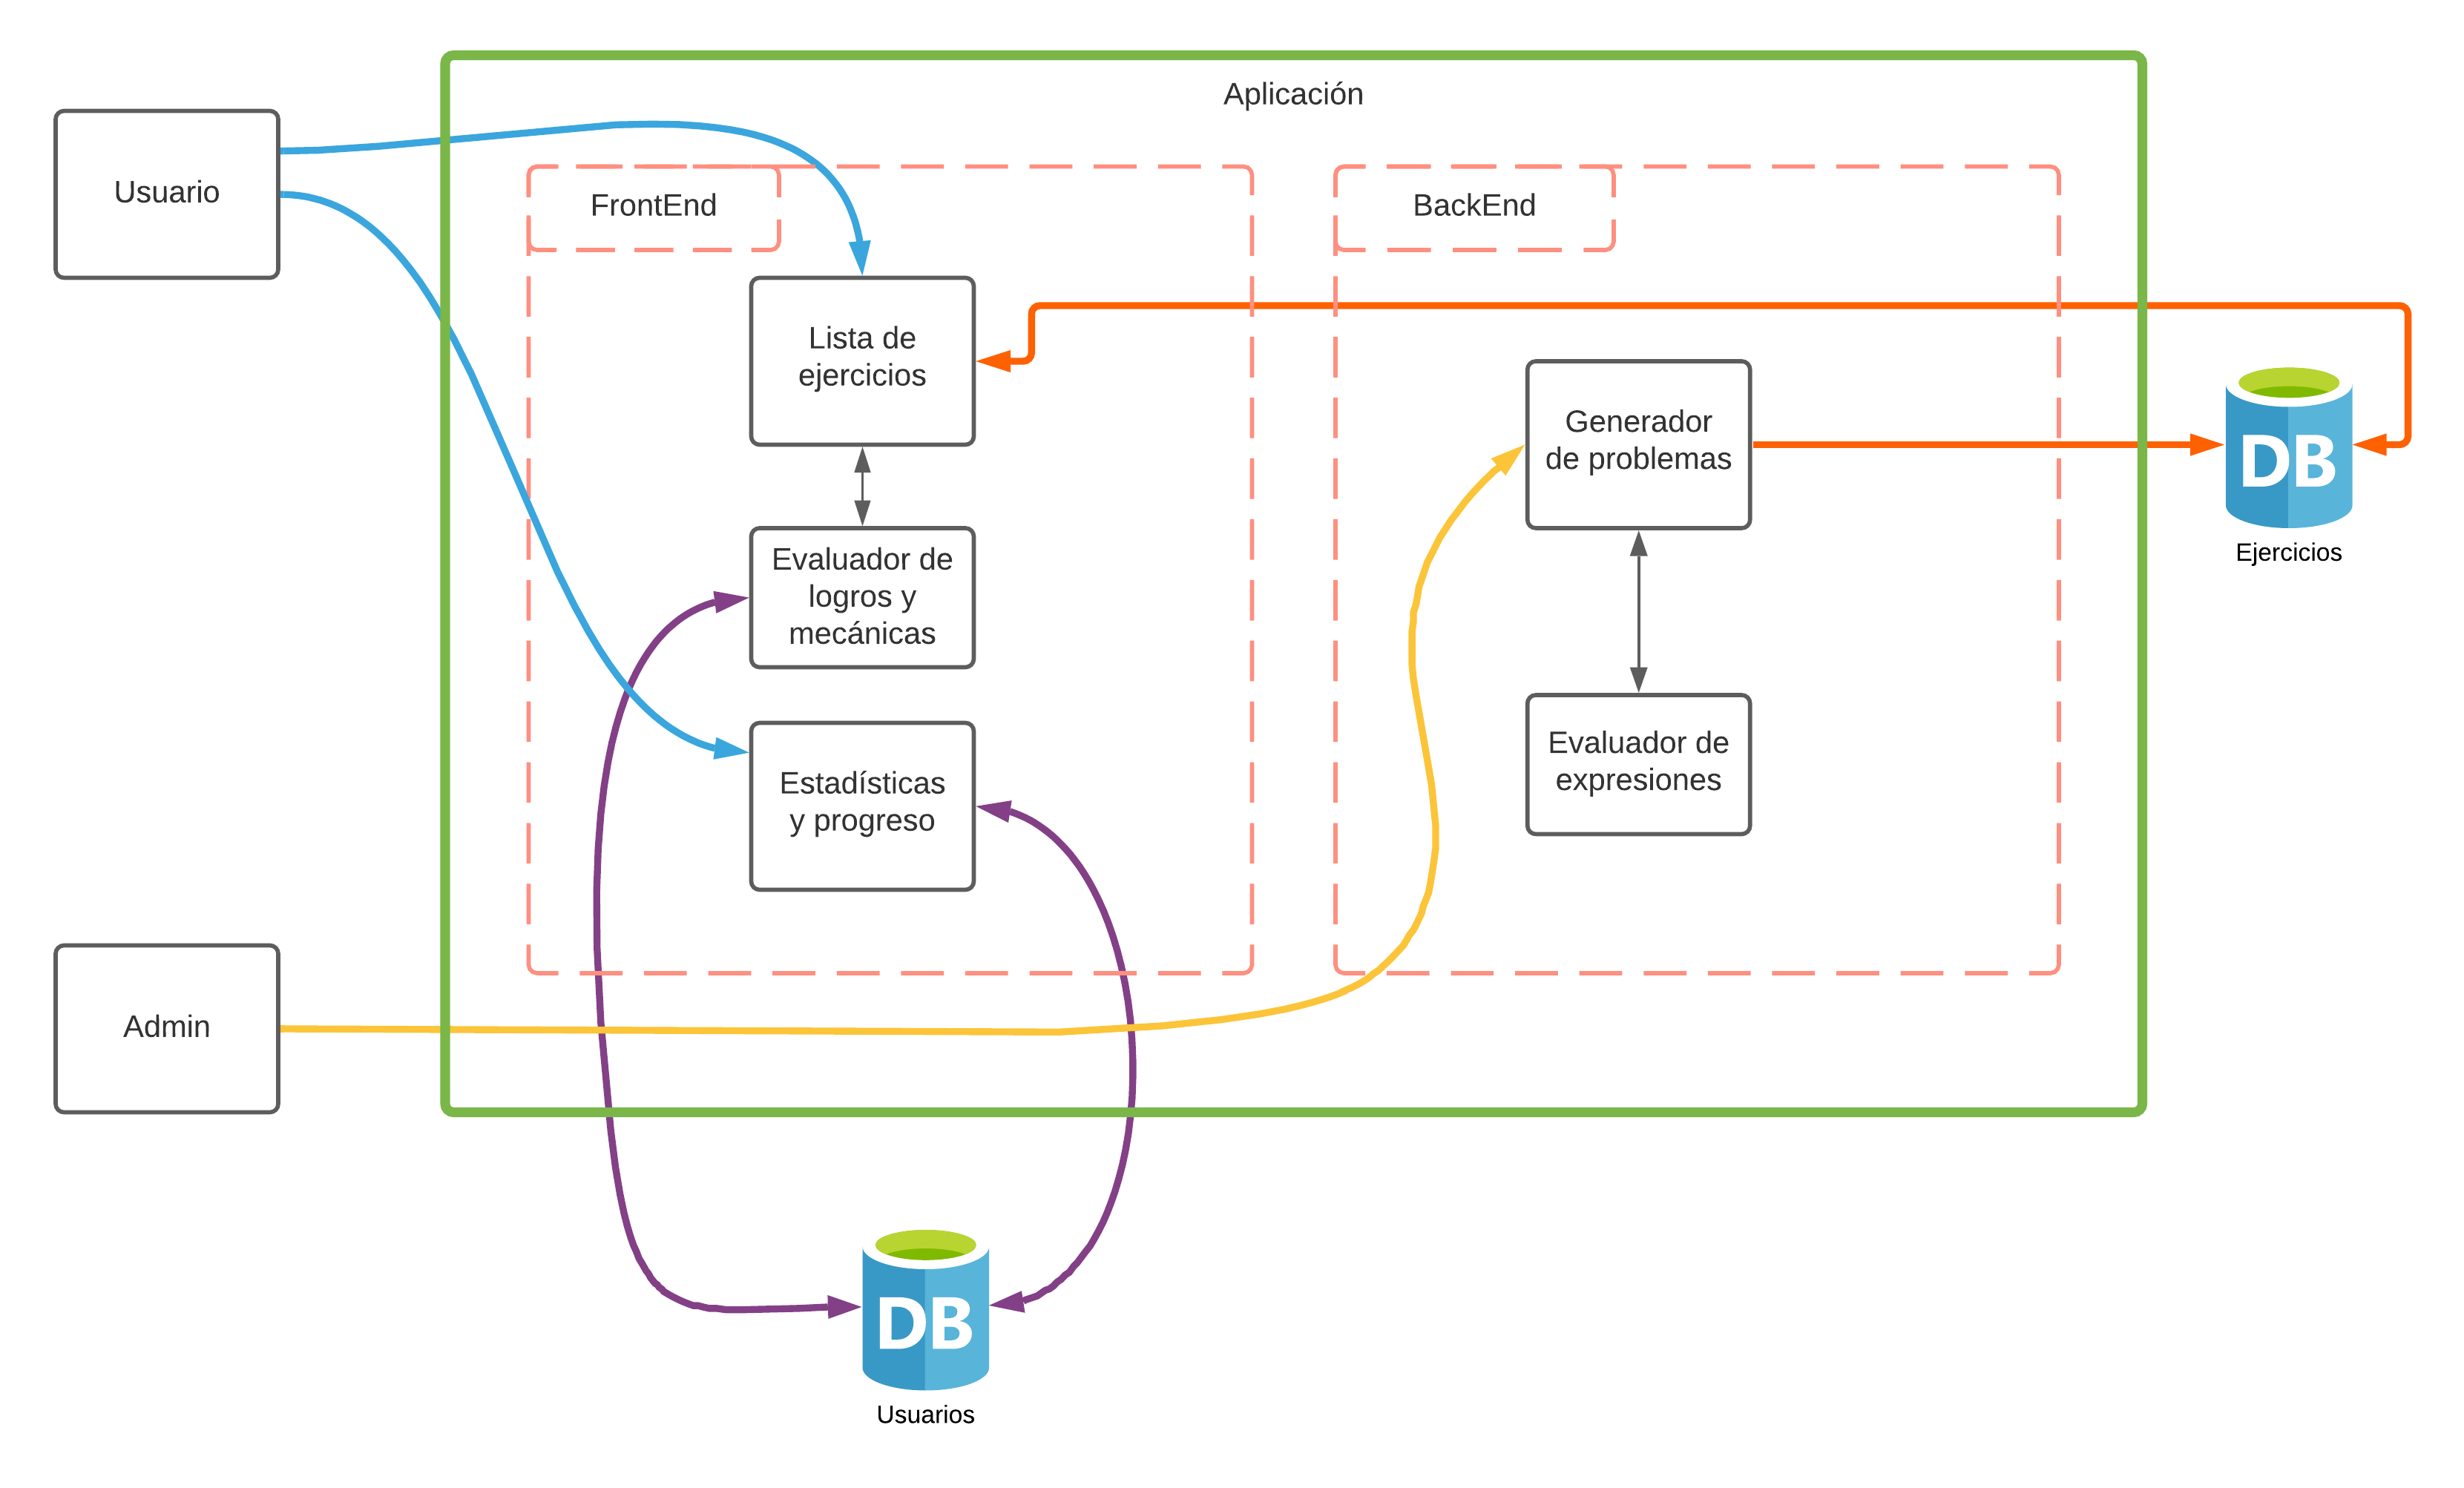
\includegraphics[width=1\textwidth]{img/diagrama_arquitectura.png}\\
\caption{Diagrama de arquitectura de la aplicación}
\label{fig:arquitectura}
\end{figure}



\section{Metodología}
La metodología que se ha elegido para el desarrollo de este proyecto es Feature planninig\cite{hunt2006feature}, 
también conocida como Feature Driven Development F.D.D Esta metodología iterativa 
orientada a objetos, consistente en planear la estructura general del proyecto, 
realizar una lista de características, planear y finalmente construir cada una de ellas. 
En nuestro caso podemos ver cada característica como un tema y ciertas funcionalidades 
adicionales que deseamos integrar. Para garantizar la variedad de ejercicios se pretende 
usar técnicas de generación por procedimientos.

La lista de características sería la siguiente:
\begin{enumerate}
	\item Sistema de puntuación
	\item Ejercicios de operaciones básicas con números enteros
	\begin{enumerate}
		\item Adición
		\item Sustracción
		\item Multiplicación
		\item División
	\end{enumerate}
	\item Ejercicios de operaciones básicas con números racionales(fracciones)
	\begin{enumerate}
		\item Adición
		\item Sustracción
		\item Multiplicación
		\item División
	\end{enumerate}
	\item Evaluador de expresiones
	\item Niveles de dificultades
	\item Leaderboards
	\item Títulos, Iconos para desbloquear con puntos
	\item Estadísticas del jugador
\end{enumerate}

\section{Cronograma}

\begin{table}[H]
\centering
\def\arraystretch{1.5}
\begin{tabular}{|M{5cm}|c|c|c|c|c|c|}
\hline
\multicolumn{1}{|c|}{Nombre:} &\multicolumn{6}{|c|}{Pineda Vieyra Itzcoatl Rodrigo}  \\\hline
\multicolumn{7}{|c|}{Título del TTR: Aplicación móvil gamificada de aritmética}\\\hline
Actividad & Agosto & Septiembre & Octubre & Noviembre & Diciembre & Enero \\\hline
Revisión de la lectura especializada en Matemática educativa 
&\cronograma& & & & & \\\hline

Definición de requerimientos
&\cronograma& & & & & \\\hline

Revisión de features
&\cronograma & & & & & \\\hline

Planeación de features
&\cronograma{}& & & & & \\\hline

Diseño de features
&\cronograma{} & & & & & \\\hline

Diseño y documentación de casos de uso
& &\cronograma{} & & & & \\\hline

Diseño de interfaz gráfica
& &\cronograma{} & & & & \\\hline

Diseño y planeación de problemas
& &\cronograma{} & & & & \\\hline

Planeación de pruebas al sistema
& &\cronograma{} & & & & \\\hline

Documentación técnica
&\cronograma{} &\cronograma{} &\cronograma{} &\cronograma{} &\cronograma{} &\cronograma{} \\\hline

Evaluador de expresiones
& & &\cronograma{} & & & \\\hline

Generador de ejercicios de operaciones básicas
(suma, resta, multiplicación, división) con números enteros
& & &\cronograma{} & & & \\\hline

Generador de ejercicios de operaciones básicas
(suma, resta, multiplicación, división) con números racionales
& & &\cronograma{} & & & \\\hline

Modo de juego infinito
& & &\cronograma{} & & & \\\hline

Modo de juego por tiempo
& & &\cronograma{} & & & \\\hline

Modulo de registro
& & &\cronograma{} & & & \\\hline

Modulo de autecticación
& & &\cronograma{} & & & \\\hline

Integración de logros
& & & &\cronograma{} & & \\\hline

Integración de tablas de liderato
& & & &\cronograma{} & & \\\hline

Integración de elementos de personalización 
& & & &\cronograma{} & & \\\hline

Pruebas funcionales 
& & & &\cronograma{} & & \\\hline

Creación de logros y respectiva población a la base de datos
& & & & &\cronograma{} & \\\hline

Elaboración manual de usuario
& & & & &\cronograma{} & \\\hline

Evaluación TTR
& & & & & &\cronograma{} \\\hline

\end{tabular}
\end{table}

\newpage

\begin{table}[H]
\centering
\def\arraystretch{1.5}
\begin{tabular}{|M{5cm}|c|c|c|c|c|c|}
\hline
\multicolumn{1}{|c|}{Nombre:} &\multicolumn{6}{|c|}{Mothelet Delgado Izaird Alexander}  \\\hline
\multicolumn{7}{|c|}{Título del TTR: Aplicación móvil gamificada de aritmética}\\\hline
Actividad & Agosto & Septiembre & Octubre & Noviembre & Diciembre & Enero \\\hline
Revisión de la lectura especializada en Matemática educativa 
&\cronograma& & & & & \\\hline

Definición de requerimientos
&\cronograma& & & & & \\\hline

Revisión de features
&\cronograma & & & & & \\\hline

Planeación de features
&\cronograma{}& & & & & \\\hline

Diseño de features
&\cronograma{} & & & & & \\\hline

Diseño y documentación de casos de uso
& &\cronograma{} & & & & \\\hline

Diseño de interfaz gráfica
& &\cronograma{} & & & & \\\hline

Diseño y planeación de problemas
& &\cronograma{} & & & & \\\hline

Planeación de pruebas al sistema
& &\cronograma{} & & & & \\\hline

Documentación técnica
&\cronograma{} &\cronograma{} &\cronograma{} &\cronograma{} &\cronograma{} &\cronograma{} \\\hline

Evaluador de expresiones
& & &\cronograma{} & & & \\\hline

Generador de ejercicios de operaciones básicas
(suma, resta, multiplicación, división) con números enteros
& & &\cronograma{} & & & \\\hline

Generador de ejercicios de operaciones básicas
(suma, resta, multiplicación, división) con números racionales
& & &\cronograma{} & & & \\\hline

Modo de juego infinito
& & &\cronograma{} & & & \\\hline

Creación de logos e iconos 
& & &\cronograma{} & & & \\\hline

Diseño de sonido
& & &\cronograma{} & & & \\\hline

Modo de juego por tiempo
& & &\cronograma{} & & & \\\hline

Modulo de registro
& & &\cronograma{} & & & \\\hline

Modulo de autecticación
& & &\cronograma{} & & & \\\hline

Integración de logros
& & & &\cronograma{} & & \\\hline

Integración de tablas de liderato
& & & &\cronograma{} & & \\\hline

Integración de elementos de personalización 
& & & &\cronograma{} & & \\\hline

Pruebas funcionales 
& & & &\cronograma{} & & \\\hline

Creación de logros y respectiva población a la base de datos
& & & & &\cronograma{} & \\\hline

Elaboración manual de usuario
& & & & &\cronograma{} & \\\hline

Evaluación TTR
& & & & & &\cronograma{} \\\hline

\end{tabular}
\end{table}


\section{Alumnos y directores}

\begin{minipage}{.45\textwidth}
Pineda Vieyra Itzcoatl Rodrigo.- Alumno de la carrera de Ing. 
en Sistemas Computacionales en ESCOM, Especialidad Sistemas, 
Boleta: 2013090802, Tel. 5518254211, email: itzcoatlpv@gmail.com
\signature


Mothelet Delgado Izaird Alexander.- Alumno de la carrera de Ing. 
en Sistemas Computacionales en ESCOM, Especialidad Sistemas, 
Boleta: 2012010743, Tel. 5538488686, email: imotheletd1100@alumno.ipn.mx
\signature

Ruiz Ledesma Elena Fabiola. - Profesora de matemáticas en la 
ESCOM del IPN y Profesora Colegiada en el Posgrado. Licenciatura 
en Matemáticas, Maestría en ciencias, especialidad Matemática y 
Educativa y Doctorado en ciencias con la misma especialidad (CINVESTAV-IPN). 
Áreas de interés: Computó educativo, Matemática Educativa. Tel: 5729 6000 ext. 
52049, email:elenfruiz65@gmail.com
\signature

Chavarría Báez Lorena. - Profesora del Departamento de Ingeniería en 
Sistemas Computacionales de la ESCOM – IPN. Doctora en Ciencias en 
Ingeniería Eléctrica opción Computación por el CINVESTAV – IPN. Áreas de 
interés: Bases de Datos, Sistemas de Información. Tel: 5729 6000 ext. 52048, 
email: lorena\_chavarria@yahoo.com.mx
\signature
	
\end{minipage}%
\hfill
\begin{minipage}{.4\textwidth}
\begin{tabular}{p{\textwidth}}
CARÁCTER: Confidencial FUNDAMENTO LEGAL: Artículo 11 Fracc. V y Artículos 108, 113 
e 117 de la Ley Federal de Transparencia y Acceso a la Información Pública. PARTES 
CONFIDENCIALES: Número de boleta y teléfono.
\end{tabular}
\end{minipage}
	

%\printbibliography[title={Bibliografía}]
\printbibliography
\end{document}